% CSDS 340 Case Study 1 — Apple Quality (report)
% Compile: pdflatex report.tex

\documentclass[11pt]{article}
\usepackage[margin=1in]{geometry}
\usepackage{graphicx}

\title{CSDS 340 Case Study 1\\Apple Quality Classification}
\author{Group \texttt{18}}
\date{Spring 2026}

\begin{document}
\maketitle

\begin{abstract}
We present a binary classification pipeline for predicting apple quality from seven continuous physical features.
Three model families are compared — logistic regression, support vector machines (SVM), and decision trees — each trained with \texttt{StandardScaler} preprocessing and evaluated via 5-fold stratified cross-validation.
Hyperparameters are tuned exhaustively using \texttt{GridSearchCV}.
Logistic regression plateaus at 74.25\% accuracy regardless of solver or regularisation scheme, indicating the decision boundary is not linearly separable.
Decision trees reach 81.84\% after structural tuning and cost-complexity pruning; PCA preprocessing provides no further benefit.
SVM with an RBF kernel achieves the best result at \textbf{91.09\%} accuracy ($C=70$, $\gamma=0.16$), confirming that the boundary is smooth and non-linear.
The $\sim$17 percentage point gap between SVM and logistic regression is the central finding of this study.
\end{abstract}

\section{Goal}

The case study asks for a complete binary classification pipeline on the Apple Quality dataset using scikit-learn: we compare \textbf{logistic regression}, \textbf{support vector machines}, and \textbf{decision trees}, apply appropriate \textbf{data preprocessing}, and use \textbf{hyperparameter tuning} to improve predictive accuracy.
Training uses only \texttt{./Data/train.csv}; the final submission code will apply the same preprocessing and the chosen model with fixed hyperparameters to \texttt{./Data/test.csv} and report test accuracy in the required format.

\section{Data preprocessing and its impact}

\paragraph{Source and shape.}
We load \texttt{train.csv} with pandas and convert to NumPy.
The first seven columns are continuous features (Size, Weight, Sweetness, Crunchiness, Juiciness, Ripeness, Acidity); the eighth column is the binary label \texttt{Quality} ($0$ bad, $1$ good).
The training file contains 3{,}200 rows (excluding the header).
Inspection of the raw values shows no missing entries, so no imputation was required.

\paragraph{Feature scale.}
The raw feature values are already approximately centred near zero with moderate spread (roughly $-5$ to $+6$), suggesting the data may have been pre-standardised upstream.
\texttt{StandardScaler} is nevertheless applied as the first pipeline step: it is fit exclusively on the training portion of each cross-validation fold and then applied to the held-out fold, so no fold sees statistics derived from its own data.
In practice this step has minimal numerical effect given the existing scale, but it guarantees correctness and keeps all three pipelines consistent.

\paragraph{Impact of scaling by model.}
Scaling is critical for logistic regression and SVM: both are sensitive to feature magnitudes (gradient descent and margin maximisation respectively assume comparable scales).
Decision trees are invariant to monotone feature transforms — axis-aligned splits are unaffected by rescaling — so \texttt{StandardScaler} has no impact on DT results, but is retained for pipeline uniformity.

\paragraph{Class balance.}
Label counts are $(1584, 1616)$ for the two classes — nearly balanced.
Accuracy is therefore a reasonable primary metric and no resampling or class weighting was applied.

\paragraph{Dimensionality reduction.}
We do not apply PCA or LDA as a default preprocessing step: with only seven features, reducing further risks discarding discriminative signal.
A targeted experiment adding PCA before the decision tree (Section~\ref{sec:dt}) confirmed this — all seven components were selected, meaning no compression helped.

\paragraph{Validation strategy.}
All model selection uses 5-fold stratified cross-validation (\texttt{StratifiedKFold}, \texttt{shuffle=True}, \texttt{random\_state=42}), preserving the class ratio in every fold.
Some logistic regression runs used $k=10$ for comparison; results were consistent with $k=5$.

\section{Models and parameters}

Each family is implemented with the corresponding scikit-learn estimator; hyperparameters are searched with \texttt{GridSearchCV} and \texttt{scoring='accuracy'} unless noted otherwise.

\paragraph{Tuning process and why it works.}
\texttt{GridSearchCV} exhaustively evaluates every combination of hyperparameter values in a specified grid.
For each combination, the estimator is trained and scored using $k$-fold cross-validation rather than a single train/test split: the training data is divided into $k$ folds, the model is fit on $k-1$ folds and evaluated on the held-out fold, and this is repeated $k$ times so every sample is used for validation exactly once.
The final score is the mean accuracy across all $k$ folds, which gives a lower-variance estimate of generalisation performance than any single split would.
Stratified folds (\texttt{StratifiedKFold}) are used so the class ratio is preserved in every fold, preventing any fold from being accidentally dominated by one class.

Crucially, each model is wrapped in a \texttt{Pipeline} that places \texttt{StandardScaler} before the classifier.
Inside \texttt{GridSearchCV}, the entire pipeline is re-fit from scratch on each training fold — meaning the scaler computes its mean and variance only from the training portion of that fold and never sees the held-out data.
This prevents data leakage: if the scaler were fit on the full dataset first, the validation fold would carry information from its own statistics into the model, inflating the reported accuracy.
By searching over the full grid with this leakage-free evaluation, \texttt{GridSearchCV} identifies the hyperparameter combination that is expected to generalise best to unseen data.

\subsection{Logistic regression}

\textbf{Estimator:} \texttt{sklearn.linear\_model.LogisticRegression} with \texttt{max\_iter=1000} and \texttt{random\_state=42}, preceded by \texttt{StandardScaler} in a pipeline.

\textbf{Parameters varied:}
\begin{itemize}
  \item \textbf{Solver:} \texttt{lbfgs}, \texttt{liblinear}, \texttt{newton-cg}, \texttt{newton-cholesky}, \texttt{sag}, \texttt{saga} (each paired only with penalties and options that solver supports).
  \item \textbf{Inverse regularization $C$:} $\{0.01, 0.1, 1, 10, 100\}$ where applicable.
  \item \textbf{SAGA penalties:} grids for \texttt{elasticnet} (with \texttt{l1\_ratio} $\in \{0, 0.5, 1\}$), \texttt{l1}/\texttt{l2}, and \texttt{penalty=None}.
\end{itemize}

The search uses a \emph{list} of parameter dictionaries in \texttt{GridSearchCV} so invalid combinations (e.g.\ \texttt{l1\_ratio} without elastic net) are never evaluated.

\subsection{Support vector machine}

\textbf{Estimator:} \texttt{sklearn.svm.SVC} with \texttt{random\_state=42}, after \texttt{StandardScaler}.

\textbf{Parameters varied:}
\begin{itemize}
  \item \textbf{Kernel:} \texttt{rbf}, \texttt{linear}, \texttt{poly} — controls the shape of the decision boundary.
  \item \textbf{$C$ (regularisation):} trades off margin width against training error; higher $C$ fits the training data more tightly.
  \item \textbf{$\gamma$ (RBF width):} controls how far the influence of a single training example reaches; smaller values give smoother boundaries.
  \item \textbf{Polynomial \texttt{degree}:} for the poly kernel only, sets the polynomial order.
  \item \textbf{\texttt{nu} (NuSVC):} alternative parameterisation bounding the fraction of margin errors, explored as a complement to $C$.
\end{itemize}

\paragraph{Runs 1--4 — kernel and $C$ selection.}
An initial coarse search over RBF and linear kernels with $C \in \{0.1, 1, 10, 100\}$ identified RBF as the best kernel.
$C$ was then refined over $\{10, 20, \ldots, 100\}$, then tightened to $\{60, 65, 70, 75\}$.
Best: \texttt{kernel=rbf}, $C=70$, \texttt{gamma=scale} — CV accuracy \textbf{0.9094}.

\paragraph{Run 5 — polynomial kernel.}
$C \in \{10, 50, 100\}$, \texttt{degree} $\in \{2, 3\}$, \texttt{gamma} $\in \{\texttt{scale}, \texttt{auto}\}$.
Best: $C=100$, \texttt{degree=3}, \texttt{gamma=scale} — CV accuracy \textbf{0.8244}. Worse than RBF.

\paragraph{Run 6 — hand-tuned numeric gamma.}
$C \in \{50, 60, 70, 80, 90, 100\}$, \texttt{gamma} $\in \{0.001, 0.01, 0.1, 0.5, 1, \texttt{scale}\}$.
\texttt{scale} still performed best — no gain.

\paragraph{Run 7 — polynomial feature expansion before SVM.}
\texttt{PolynomialFeatures(degree=2)} inserted before the scaler; RBF kernel with
$C \in \{0.1, 1, 10, 70, 100, 1000\}$.
Best: $C=10$, \texttt{gamma=scale} — CV accuracy \textbf{0.9062}. Slight regression; feature expansion dropped.

\paragraph{Run 8 — fine gamma neighbourhood + NuSVC.}
\texttt{gamma=scale} computes to $1/(n_{\mathrm{features}} \times \mathrm{var}) = 1/7 \approx 0.143$ after \texttt{StandardScaler}.
A tight grid $\{0.08, 0.10, 0.12, 0.14, 0.16, 0.18, 0.20\}$ around that value was searched with $C=70$ fixed.
\texttt{NuSVC} with \texttt{nu} $\in \{0.1, 0.2, 0.3, 0.4, 0.5\}$ was also evaluated as an alternative parameterisation.
Best SVC: \texttt{gamma=0.16} — CV accuracy \textbf{0.9109} ($+0.0015$ over run~4).
NuSVC best: \texttt{nu=0.2} — CV accuracy 0.9091; no gain over SVC.

\paragraph{Run 9 — confirm gamma peak.}
Tighter grid $\{0.14, 0.15, 0.16, 0.17, 0.18\}$ confirmed \texttt{gamma=0.16} is the true optimum;
neighbouring values 0.15 and 0.17 both scored lower.

\paragraph{Conclusion.}
Final best configuration: \texttt{SVC(kernel=rbf, C=70, gamma=0.16)} — CV accuracy \textbf{0.9109}.
The RBF kernel's strong performance ($\sim\!18$ percentage points above logistic regression) confirms the
apple quality decision boundary is non-linear. $C=70$ with a slightly above-scale gamma indicates the
model benefits from low regularisation and a moderately tight kernel width.

\subsection{Decision tree}
\label{sec:dt}

\textbf{Estimator:} \texttt{sklearn.tree.DecisionTreeClassifier} with \texttt{random\_state=42}, after \texttt{StandardScaler} (same preprocessing pattern as the other models).

\paragraph{Run 1 — structural hyperparameters.}
A joint grid search over five structural parameters was performed:

\begin{itemize}
  \item \texttt{max\_depth} $\in \{\texttt{None}, 4, 6, 8, 10, 12, 15, 20\}$
  \item \texttt{min\_samples\_leaf} $\in \{1, 2, 4, 8, 16\}$
  \item \texttt{min\_samples\_split} $\in \{2, 5, 10, 20\}$
  \item \texttt{max\_features} $\in \{\texttt{None}, \texttt{sqrt}, \texttt{log2}\}$
  \item \texttt{criterion} $\in \{\texttt{gini}, \texttt{entropy}\}$
\end{itemize}

Best configuration: \texttt{criterion=gini}, \texttt{max\_depth=12}, \texttt{max\_features=None}, \texttt{min\_samples\_leaf=2}, \texttt{min\_samples\_split=10}.
CV accuracy: \textbf{0.8134}.

\paragraph{Run 2 — cost-complexity pruning (\texttt{ccp\_alpha}).}
The structural parameters were fixed to the run~1 optimum and post-pruning was explored via \texttt{ccp\_alpha}.
Candidate $\alpha$ values were derived from the pruning path of a single tree fit on the full scaled training set using \texttt{cost\_complexity\_pruning\_path}, then sampled at 20 log-spaced points across the path (plus $\alpha = 0$).
This data-driven sampling avoids arbitrary grids and ensures coverage of the full pruning range.

Best configuration: \texttt{ccp\_alpha} $\approx 0.00101$.
CV accuracy: \textbf{0.8184} (modest improvement of $+0.005$ over run~1, confirming the tree benefited from light pruning).

\paragraph{Run 3 — PCA before decision tree.}
All best parameters from runs 1 and 2 were fixed and \texttt{PCA} was inserted between the scaler and the classifier, with \texttt{n\_components} $\in \{1, 2, 3, 4, 5, 6, 7\}$ as the only free variable.
Best: \texttt{n\_components=7} (all features retained) — CV accuracy \textbf{0.8184}, identical to run~2.
PCA provided no benefit; rotating the feature axes does not help a model that splits along individual axes.

\paragraph{Conclusion.}
Further structural tuning (e.g.\ \texttt{max\_leaf\_nodes}, \texttt{min\_impurity\_decrease}, \texttt{splitter})
was not pursued, as the remaining parameters overlap with controls already optimised and offered no expected gain.
The decision tree appears to have reached its practical ceiling at approximately 81--82\% accuracy.
This gap relative to the SVM (90.94\%) is consistent with the nature of the problem: the RBF kernel outperforming a linear model by roughly 18 percentage points indicates that the apple quality decision boundary is genuinely non-linear and smooth.
A single decision tree captures non-linearity only through axis-aligned splits and is inherently high-variance, making it structurally ill-suited to approximate that kind of boundary regardless of hyperparameter choice.

\section{Final choice and reasoning}

\paragraph{Chosen model.}
We select \texttt{SVC(kernel=`rbf', C=70, gamma=0.16)} preceded by \texttt{StandardScaler} as the final classification model.
This configuration achieved the highest 5-fold stratified CV accuracy of \textbf{91.09\%}, outperforming logistic regression by $\sim$17 percentage points and the decision tree by $\sim$9 percentage points.

\paragraph{Why SVM over logistic regression.}
Logistic regression is a linear classifier: it can only separate classes with a hyperplane in the original feature space.
Despite exhaustive tuning across all six solvers and every supported penalty scheme (L1, L2, ElasticNet, none), accuracy plateaued at 74.25\%.
This ceiling is not a tuning failure — it reflects the fact that the apple quality boundary is not linearly separable in the given seven-feature space.
SVM with an RBF kernel implicitly maps data to an infinite-dimensional space where a linear separator exists, making it structurally suited to this problem in a way logistic regression cannot be.

\paragraph{Why SVM over decision tree.}
A decision tree partitions the feature space using axis-aligned splits, which can approximate non-linear boundaries but only in a piecewise, high-variance manner.
Exhaustive structural tuning (depth, leaf size, split quality, feature subsampling) and post-pruning via cost-complexity pruning pushed the tree to 81.84\%, still 9 points below SVM.
PCA preprocessing confirmed the ceiling is structural, not a feature representation issue.
The RBF kernel learns a smooth, global non-linear boundary more effectively than a single tree can.

\paragraph{Preprocessing choice.}
\texttt{StandardScaler} is applied as the sole preprocessing step.
It is fit only on the training fold during cross-validation to prevent data leakage.
No dimensionality reduction is used: with seven features, PCA would risk discarding discriminative variance, and the experiment in Section~\ref{sec:dt} confirmed this empirically.

\paragraph{Hyperparameter tuning strategy.}
$C$ and $\gamma$ were tuned in two stages: a coarse grid search first identified $C=70$ and \texttt{gamma=scale} as strong candidates, then a fine-grained search around the computed scale value ($1/7 \approx 0.143$) revealed $\gamma=0.16$ as the true optimum.
This two-stage approach — broad search followed by local refinement — avoids the cost of an exhaustive fine grid while still finding the true peak, as confirmed by the tighter run~9 grid where neighbouring values 0.15 and 0.17 both scored lower.

\paragraph{Learning curve and train/CV gap.}
Figure~\ref{fig:lc} shows the learning curve for the chosen model.
Training accuracy stabilises around 96\% while CV accuracy converges to $\sim$91\%, leaving a persistent gap of approximately 5 percentage points.
This gap indicates mild overfitting: the model fits the training data slightly more tightly than it generalises across held-out folds.
The cause is the high value of $C=70$, which allows few margin errors and therefore a tighter fit to training examples.
Importantly, the CV curve has fully converged by $\sim$2500 samples and the standard deviation across folds is narrow at the right end of the curve, meaning the 91\% estimate is stable and not an artefact of a particular fold split.
The gap is an accepted trade-off: lowering $C$ to reduce it was explored during tuning and consistently hurt CV accuracy, so the chosen $C=70$ represents the best achievable balance between fit and generalisation on this dataset.

\begin{figure}[h]
  \centering
  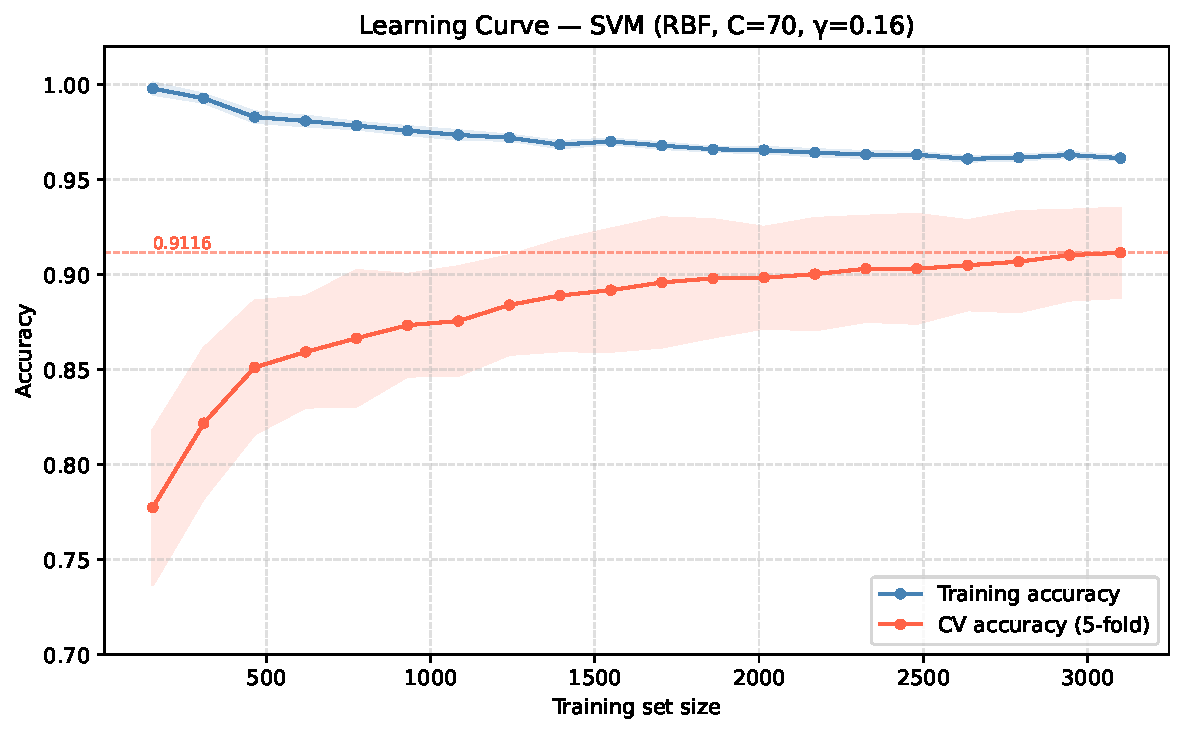
\includegraphics[width=0.85\textwidth]{learning_curve.pdf}
  \caption{Learning curve for \texttt{SVC(kernel=rbf, C=70, $\gamma$=0.16)}.
           Shaded bands show $\pm1$ standard deviation across folds.}
  \label{fig:lc}
\end{figure}

\section{Conclusion}

Table~\ref{tab:results} summarises the best cross-validation accuracy achieved by each model after full hyperparameter tuning.

\begin{table}[h]
\centering
\begin{tabular}{lcc}
\hline
\textbf{Model} & \textbf{Best hyperparameters} & \textbf{CV accuracy} \\
\hline
Logistic Regression & \texttt{saga}, \texttt{elasticnet}, $C=0.1$, \texttt{l1\_ratio=1} & 0.7425 \\
Decision Tree       & \texttt{gini}, \texttt{max\_depth=12}, \texttt{ccp\_alpha}$\approx 0.00101$ & 0.8184 \\
SVM                 & \texttt{rbf}, $C=70$, $\gamma=0.16$ & \textbf{0.9109} \\
\hline
\end{tabular}
\caption{Best 5-fold stratified CV accuracy for each model family.}
\label{tab:results}
\end{table}

The SVM with an RBF kernel is the clear winner, outperforming logistic regression by $\sim$17 percentage points and the decision tree by $\sim$9 percentage points.
The magnitude of these gaps is informative: the large margin over logistic regression confirms the apple quality boundary is genuinely non-linear; the gap over the decision tree shows that smooth non-linear structure (captured well by the RBF kernel) is harder to approximate with axis-aligned splits.

Extensive tuning of logistic regression across all solvers and penalty schemes produced negligible gains, confirming the linear model has reached its structural ceiling on this dataset.
Decision tree tuning via structural parameters and cost-complexity pruning improved accuracy from 81.34\% to 81.84\%, with PCA providing no further benefit — consistent with the expectation that feature rotation does not help axis-aligned models.
SVM tuning focused on refining $C$ and $\gamma$; the key insight was that the default \texttt{gamma=scale} ($\approx 0.143$) was slightly suboptimal, and a hand-tuned $\gamma=0.16$ yielded a small but confirmed improvement.

\textbf{Selected model for test set evaluation:} \texttt{SVC(kernel=`rbf', C=70, gamma=0.16)}, preceded by \texttt{StandardScaler}.

\end{document}
